\documentclass[tikz, border=3mm]{standalone}
\usepackage{tikz}
\usepackage{amsmath} % For \operatorname
\usepackage{amssymb} % For \mathbb
\usetikzlibrary{patterns.meta} % For patterns

\begin{document}
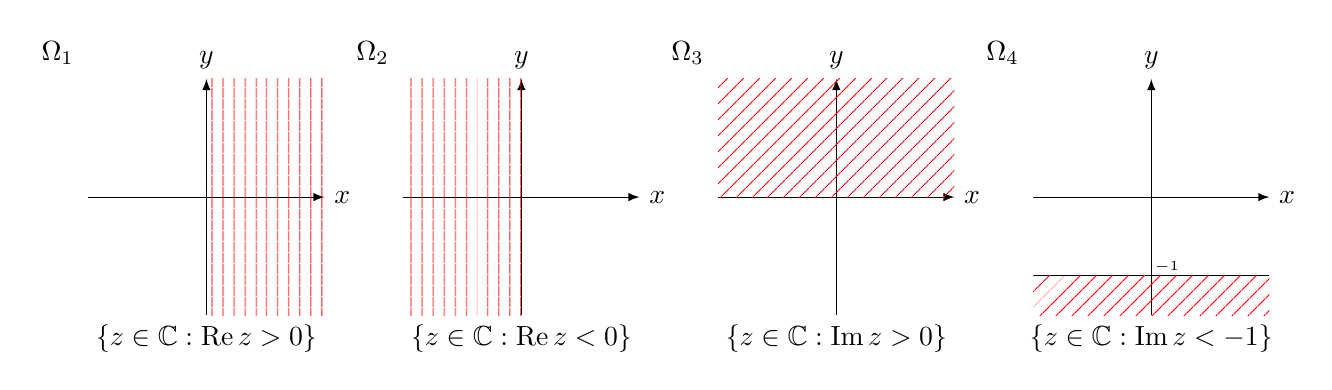
\begin{tikzpicture}[
    % Define axis style
    axis/.style={->, >=latex},
    % Define hatch styles
    hatch vert/.style={pattern={Lines[angle=90, distance=4pt]}, pattern color=red},
    hatch diag/.style={pattern={Lines[angle=45, distance=4pt]}, pattern color=red},
    plotlabel/.style={above left, inner sep=5pt},
    description/.style={below, align=center, node distance=0.5cm} % Style for text below plots
]

% Common axis limits
\def\xmin{-1.5}
\def\xmax{1.5}
\def\ymin{-1.5}
\def\ymax{1.5}

% Plot 1: Omega_1 (Re z > 0)
\begin{scope}
    \draw[axis] (\xmin,0) -- (\xmax,0) node[right] {$x$};
    \draw[axis] (0,\ymin) -- (0,\ymax) node[above] {$y$};
    \node[plotlabel] at (\xmin,\ymax) {$\Omega_1$};
    \fill[hatch vert] (0,\ymin) rectangle (\xmax,\ymax);
    \node[description] at (0,\ymin) {$\{z \in \mathbb{C} : \operatorname{Re} z > 0\}$};
\end{scope}

% Plot 2: Omega_2 (Re z < 0)
\begin{scope}[shift={(4,0)}] % Shift right for next plot
    \draw[axis] (\xmin,0) -- (\xmax,0) node[right] {$x$};
    \draw[axis] (0,\ymin) -- (0,\ymax) node[above] {$y$};
    \node[plotlabel] at (\xmin,\ymax) {$\Omega_2$};
    \fill[hatch vert] (\xmin,\ymin) rectangle (0,\ymax);
     \node[description] at (0,\ymin) {$\{z \in \mathbb{C} : \operatorname{Re} z < 0\}$};
\end{scope}

% Plot 3: Omega_3 (Im z > 0)
\begin{scope}[shift={(8,0)}] % Shift right again
    \draw[axis] (\xmin,0) -- (\xmax,0) node[right] {$x$};
    \draw[axis] (0,\ymin) -- (0,\ymax) node[above] {$y$};
    \node[plotlabel] at (\xmin,\ymax) {$\Omega_3$};
    \fill[hatch diag] (\xmin,0) rectangle (\xmax,\ymax);
     \node[description] at (0,\ymin) {$\{z \in \mathbb{C} : \operatorname{Im} z > 0\}$};
\end{scope}

% Plot 4: Omega_4 (Im z < -1)
\begin{scope}[shift={(12,0)}] % Shift right again
    \draw[axis] (\xmin,0) -- (\xmax,0) node[right] {$x$};
    \draw[axis] (0,\ymin) -- (0,\ymax) node[above] {$y$};
    \node[plotlabel] at (\xmin,\ymax) {$\Omega_4$};
    % Draw the boundary line y=-1
    \draw (\xmin,-1) -- (\xmax,-1);
    \node[above right, font=\tiny, inner sep=1pt] at (0,-1) {$-1$}; % Label for the line
    % Fill the region below y=-1
    \fill[hatch diag] (\xmin,\ymin) rectangle (\xmax,-1);
     \node[description] at (0,\ymin) {$\{z \in \mathbb{C} : \operatorname{Im} z < -1\}$};
\end{scope}

\end{tikzpicture}
\end{document}